%\vspace*{\fill}

\begin{figure}[!htb]
	\centering
	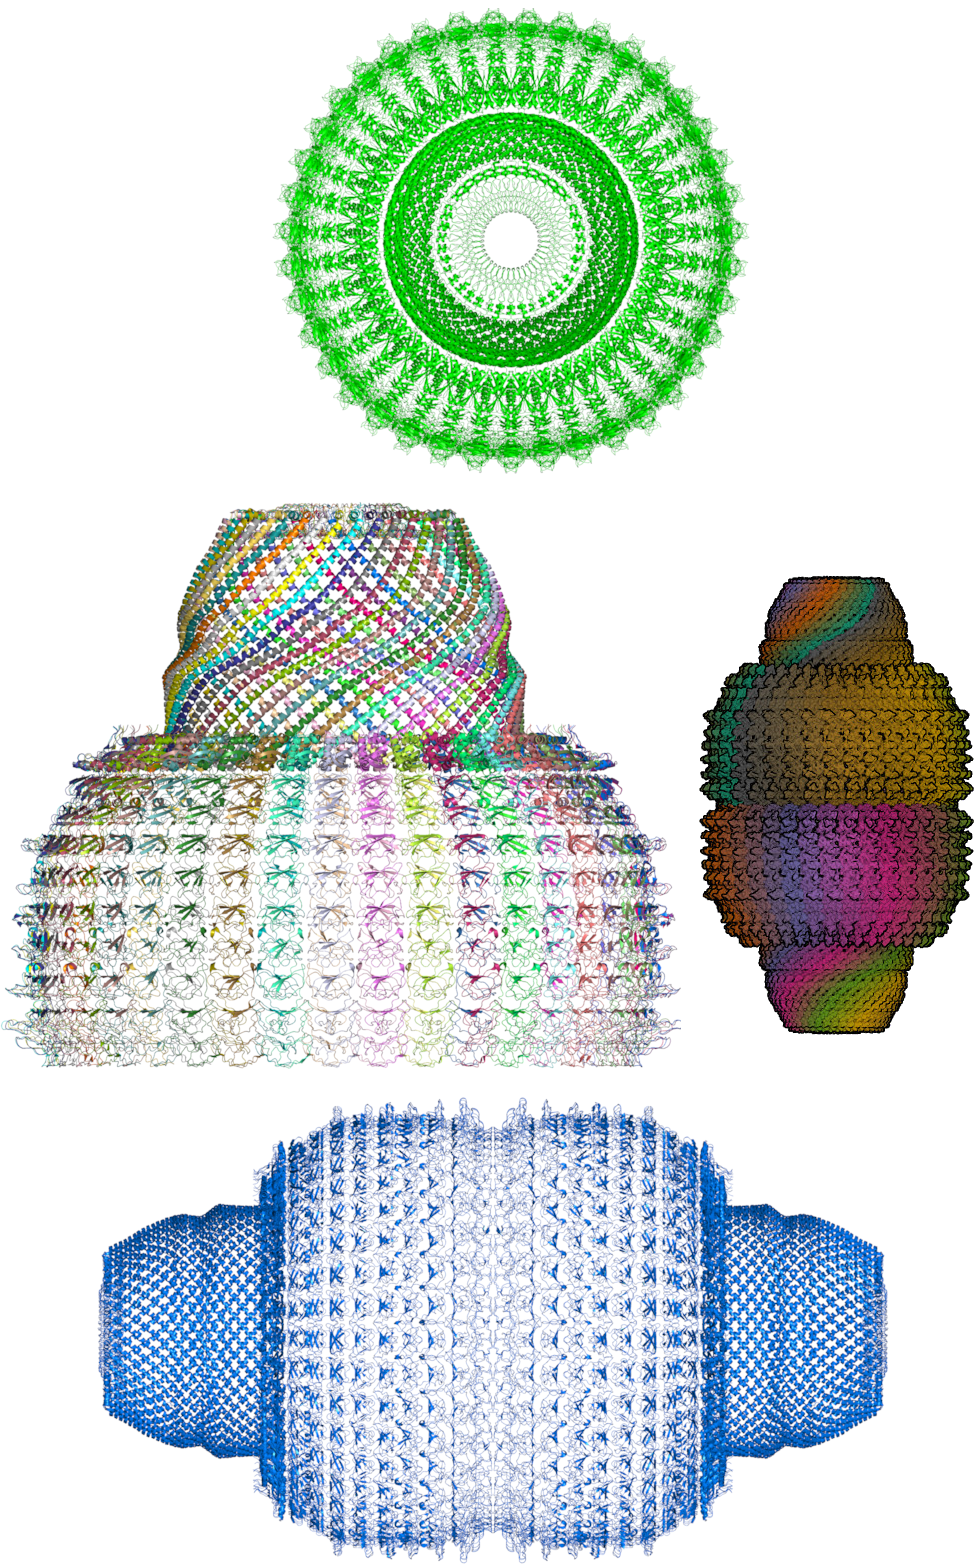
\includegraphics[scale=1.55]{images/4v60_2.png}
	\caption{Rappresentazione della struttura del "vault" (ribonucleoproteina) del fegato di ratto con una risoluzione di 3.5\angstrom, vista da varie angolazioni. La struttura di un vault è composta da 78 copie della Major Vault Protein assemblate. I "vault" sono proteine citoplasmatiche che devono il loro nome alla loro somiglianza con le "volte" di una cattedrale. Fonte\cite{4v60}}
	\label{fig:vault}
\end{figure}

%\vspace*{\fill}

\clearpage